\section{KV Cache Reconciliation across Stage Promotions}
\label{sec:kv_reconcile}

After stage promotion, the conversation context remains valid but KV states cached under the earlier configuration may no longer be semantically compatible with the promoted model. A naive fix is to evict all cached blocks and let the next request perform full prefill. This is correct, but it shifts a large recomputation penalty to the first post-promotion user interaction.

\paragraph{Boundary-based correctness criterion.}
Let $\Delta_s$ be the set of layers whose parameters change at promotion $s\!\rightarrow\!s{+}1$, and define the promotion point as
\begin{equation}
b = \min \Delta_s .
\end{equation}
Let $h^{s}_{l,t}$ denote the hidden state at layer $l$, token position $t$, and stage $s$, and let $W^{s}_l$ denote the parameters of layer $l$ at stage $s$. For any token position $t$, post-promotion KV consistency requires
\begin{equation}
(K^{s+1}_{l,t},V^{s+1}_{l,t}) =
\begin{cases}
(K^{s}_{l,t},V^{s}_{l,t}), & l < b,\\
F_l(H^{s+1}_{l-1,t}; W^{s+1}_l), & l \ge b.
\end{cases}
\label{eq:kv_boundary_rule}
\end{equation}
Layers before the promotion point are unchanged across stages, so their cached KV states can be reused directly. Layers at or beyond the promotion point either execute with changed weights or receive changed inputs, so their KV states must be recomputed under the promoted model. Figure~\ref{fig:kv-reconcile-concept} illustrates this rule for the representative Stage~1$\rightarrow$Stage~2 case: although Stage~1 already contains an active upper suffix, activating the first deferred segment changes hidden states from layer $b$ onward, making the entire later-layer suffix stale rather than only the newly activated segment itself.

% Update the path below if your conceptual figure PDF uses a different filename.
\begin{figure*}[t]
\centering
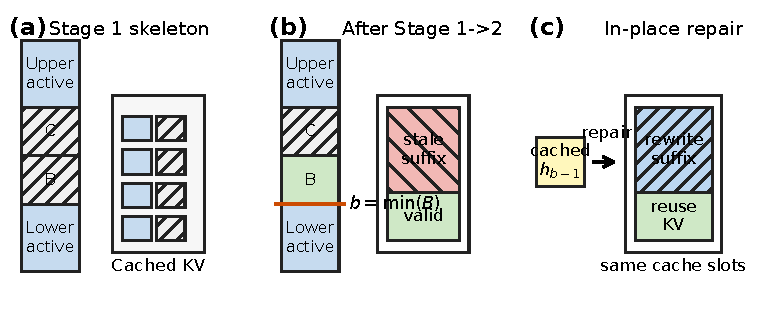
\includegraphics[width=0.97\textwidth]{kv_boundary_reconciliation}
\caption{Boundary-aware KV-cache reconciliation across stage promotions. (A) Stage~1 executes on the full-depth skeleton with active lower and upper layers while the deferred middle recovery segments remain virtual. (B) After Stage~1$\rightarrow$Stage~2 promotion, the promotion boundary $b=\min(B)$ marks the first changed layer. KV states below $b$ remain valid, whereas the later-layer suffix $b\ldots N{-}1$ becomes stale across all cached tokens. (C) On the common fast path, ProgressiveServe starts from the cached hidden state $h_{b-1}$, rewrites only the later-layer KV suffix in place, and preserves both lower-layer KV and physical cache-slot ownership. The same rule applies to Stage~2$\rightarrow$Stage~3 with $b=\min(C)$; fallback partial recompute is omitted for clarity.}
\label{fig:kv-reconcile-concept}
\end{figure*}

\paragraph{Prefix-preserving rematerialization.}
Rather than evicting all cached state, ProgressiveServe repairs only the KV entries at and beyond the promotion point. As shown in Figure~\ref{fig:kv-reconcile-concept}(C), the runtime starts from the cached hidden state at layer $b{-}1$, re-executes layers $b, \ldots, L{-}1$ under the post-promotion weights, and writes the repaired KV states back into the same physical cache slots. KV states before the promotion point remain untouched. On the common fast path, this update preserves prefix-cache mapping, so subsequent requests retain prefix hits instead of paying a full-prefix miss.

\paragraph{Integration with vLLM's prefix cache.}
Concretely, given sequence length $T$ and block size $B$, the physical slot for token position $t$ is determined by
\begin{equation}
\pi(t)=\mathrm{BT}\!\left(\left\lfloor t/B \right\rfloor\right)
\cdot B + (t \bmod B),
\label{eq:slot_mapping}
\end{equation}
where $\mathrm{BT}(\cdot)$ maps logical to physical cache blocks. Rematerialization writes repaired KV directly to $\pi(t)$ for layers $l \ge b$, preserving hash-to-block ownership so that later requests continue to benefit from prefix hits.

\paragraph{Failure-safe fallback.}
If the preconditions for prefix-preserving rematerialization are not satisfied, such as missing block metadata or insufficient saved activations, ProgressiveServe falls back to a correctness-first path: it clears the prefix cache and runs a single eager prefill over the current conversation. Layers before the promotion point execute only the minimal KV-only work needed to regenerate their entries, whereas layers at and beyond the promotion point execute full forward passes. This fallback is one-shot; subsequent steps resume normal decode.

\paragraph{Cost perspective.}
A full cache reset recomputes all $L$ layers over the entire context. Prefix-preserving rematerialization recomputes only layers $b$ through $L{-}1$, skipping all layers before the promotion point entirely. The fallback path additionally regenerates KV entries for layers before $b$, but uses a lightweight KV-only pass that is substantially cheaper than full forward execution. In both cases, the repair cost scales with the number of changed layers rather than total model depth.
